\documentclass[10pt,a4paper]{article}
\usepackage[T1]{fontenc}
\usepackage[utf8x]{inputenc}
\usepackage[italian]{babel}
\usepackage{amsmath}
\usepackage[small,bf]{caption}
\usepackage{color}
\usepackage{graphicx}
\usepackage{hyperref}
%\hypersetup{colorlinks=true}
\usepackage{url}

\author{\textbf{Candidato: }\textit{Ju Liu}\\\textbf{Relatori:
  }\textit{Fulvio Risso, Giuseppina Gini}}
\title{Analysis and implementation of a constrained path
    computation algorithm in a multi-layer GMPLS network}

\begin{document}
\maketitle

\section*{Scopo della tesi}

Lo scopo di questa tesi consiste nel progettare e realizzare un
algoritmo che calcoli percorsi di rete in un ambiente \textbf{multi-layer},
cioè composto da diverse tecnologie di rete. La soluzione
implementata permette infatti di gestire una rete complessa, composta
da elementi molto diversi tra di loro: dispositivi ottici, switch
Ethernet e router MPLS coesistono e sono gestiti dalla stessa suite di
protocolli (si veda l'esempio in Figura~\ref{fig:multi_path}).

\begin{figure}[!htbp]
  \begin{center}
    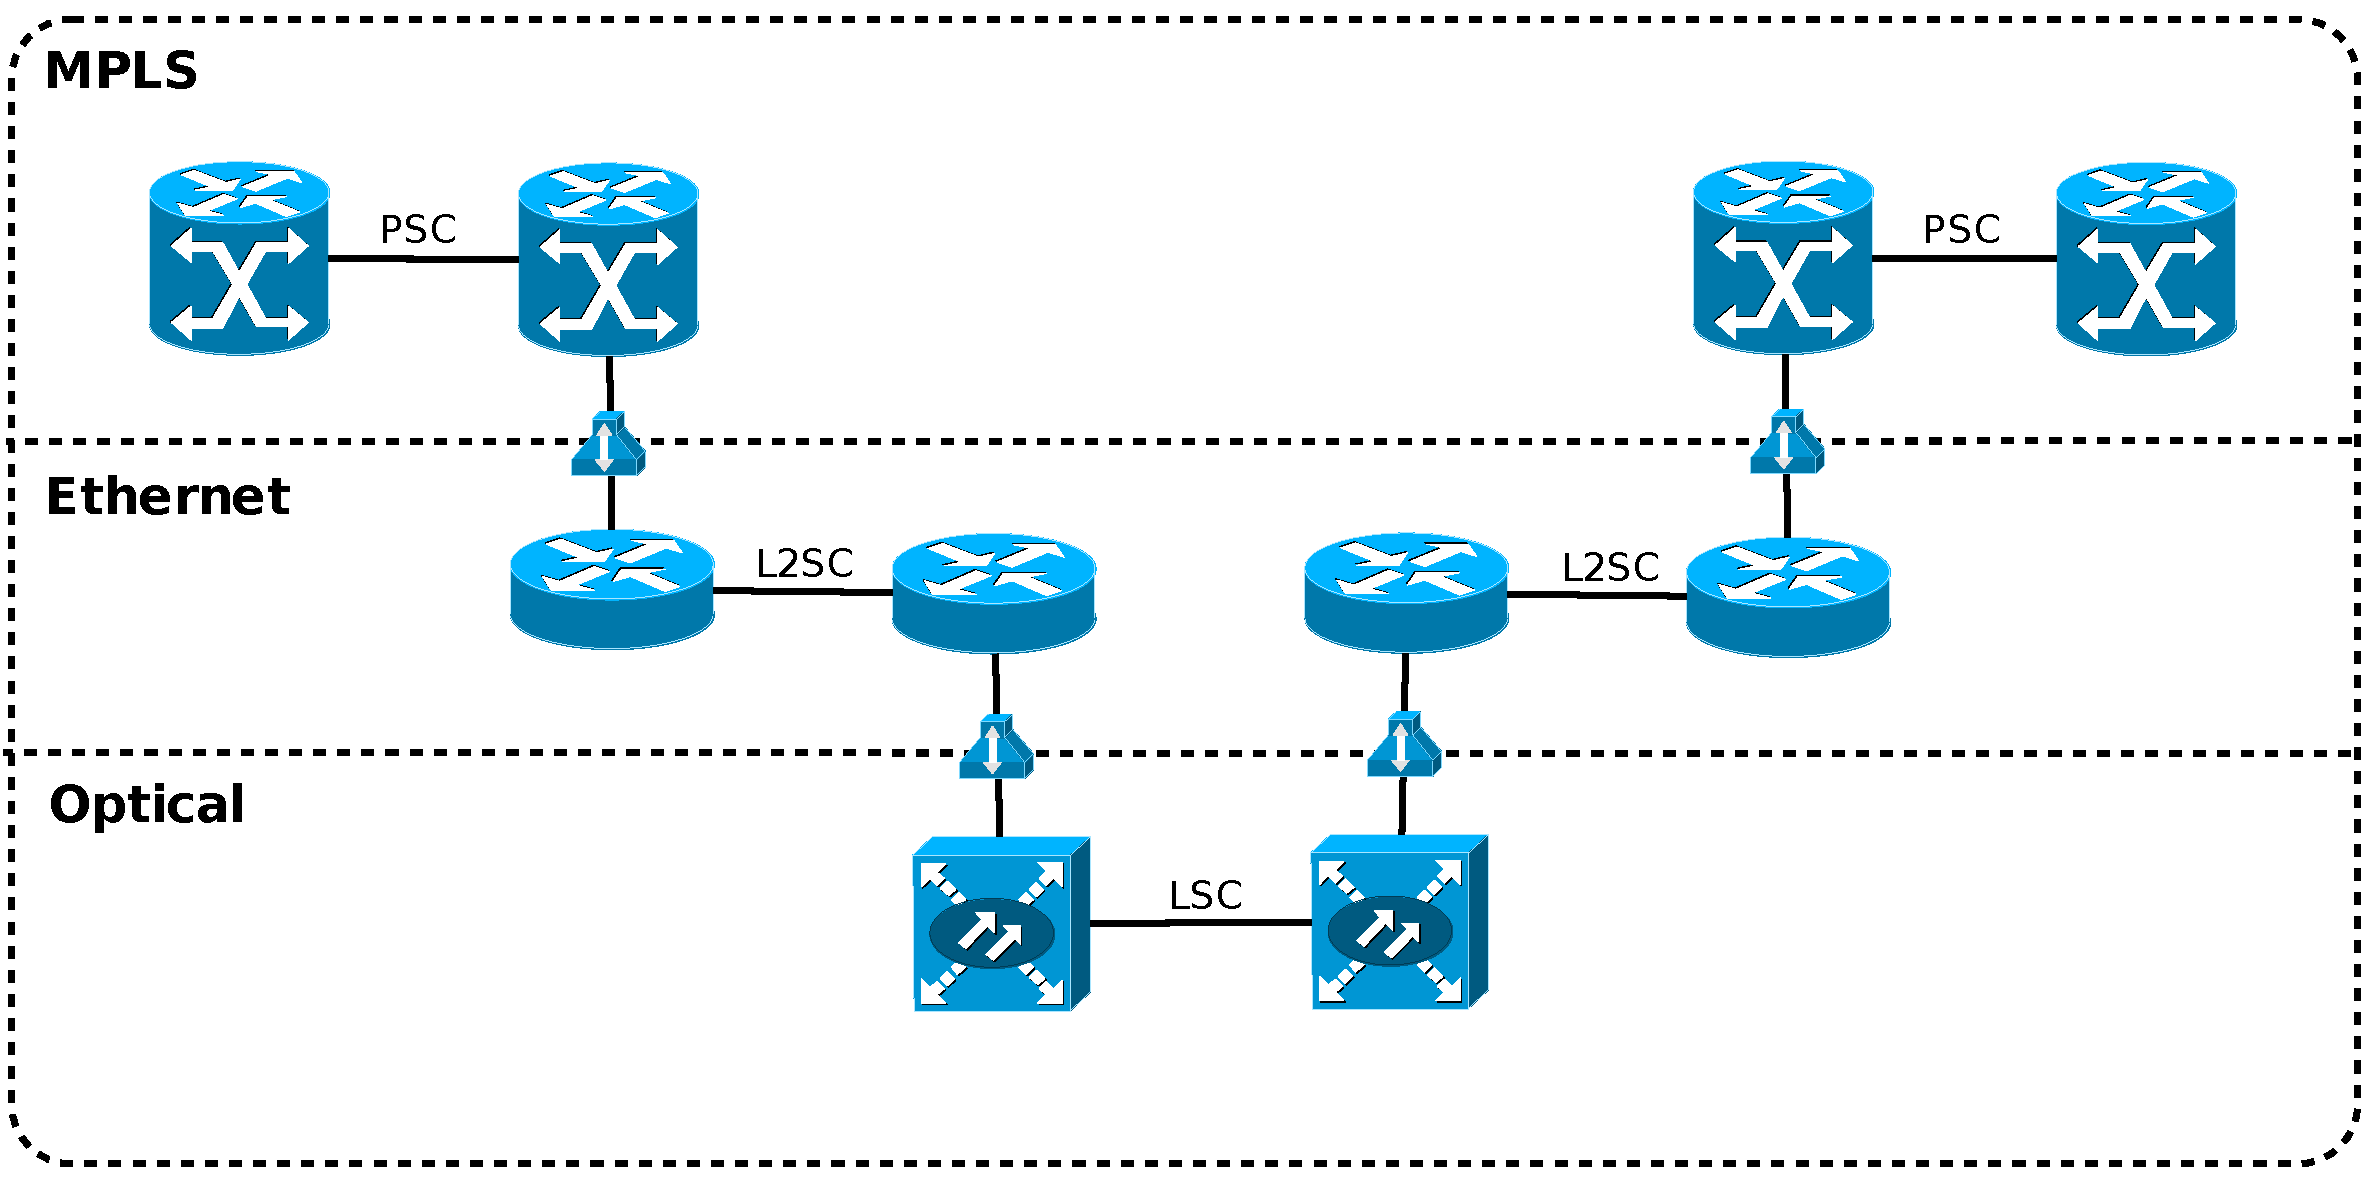
\includegraphics[width=1\textwidth]{img/multi_path}
    \caption[]{Un esempio di percorso di rete in ambiente multi-layer:
      il livello MPLS è \textit{Packet Switching Capable} (PSC),
      quello Ethernet \textit{Layer 2 Switching Capable} (L2SC) e
      quello ottico \textit{Lambda Switching Capable} (LSC).}
    \label{fig:multi_path}
  \end{center}
\end{figure}

L'algoritmo dovrà essere in grado di attraversare diverse tecnologie
di rete in maniera trasparente, calcolando il percorso ottimale che
collega una coppia di nodi; quale sia il percorso ottimale è definito
dall'utente, che nella richiesta di computazione specifica i diversi
vincoli che devono essere rispettati.

Questi vincoli possono riguardare l'intero percorso, come ad esempio
la latenza o il costo totale, o solo una parte di esso, come i vincoli
relativi al solo segmento ottico.

\section*{Ambito di ricerca}

Il campo di ricerca che è maggiormente coinvolto in questo lavoro è
quello della gestione automatica di reti complesse multi-layer, e in
particolare della possibilità di configurare le connessioni
automaticamente. Nelle reti di questo tipo, l'approccio attuale
consiste nel configurare ogni livello singolarmente e poi configurare
i vari punti di adattamento tra i livelli; tuttavia, al crescere della
dimensione delle reti e della loro complessità intrinseca, questo
lavoro può diventare molto difficile e delicato. Il meccanismo
proposto prevede una configurazione unificata in cui le differenze tra
le diverse tecnologie di rete siano gestite dal software, che risolve
questa complessità al posto dell'utente.

Un altro argomento a cui viene posta un'attenzione particolare è
quello del \textbf{traffic engineering}, che riguarda la progettazione
di meccanismi e protocolli che garantiscono un utilizzo efficiente
delle risorse di rete. In questo caso, l'algoritmo realizzato può
essere utilizzato per diversi scopi, per esempio calcolare percorsi su
cui sia garantita una \textit{Quality of Service} ben definita, oppure
generare percorsi alternativi da utilizzare in caso di congestioni
all'interno della rete.


\section*{Contributi personali}

Il candidato si è occupato della progettazione dell'algoritmo
multi-layer, della sua implementazione in C++ e del suo successivo
inserimento all'interno della piattaforma software
DRAGON\footnote{\url{http://dragon.maxgigapop.net/twiki/bin/view/DRAGON/}}:
in particolare, si è lavorato sulla versione estesa dalla ditta
svedese Acreo\footnote{\url{http://www.acreo.se}}.

Nella prima fase del progetto, si è proceduto a riscrivere sezioni di
codice, introducendo nuove classi e modificando quelle esistenti per
creare un'architettura più strutturata; grazie a questo approccio, si
è potuto in seguito sfruttare il polimorfismo delle classi per
implementare l'algoritmo con una maggiore scalabilità e flessibilità.

Completata la riscrittura del codice esistente, si è passati a
definire la struttura dell'algoritmo multi-layer, prendendo come
spunto quella degli altri moduli presenti nella piattaforma; in
seguito, sono stati ricercati e implementati i vincoli più importanti
da considerare durante la computazione.

Si è dunque proceduto a verificare la correttezza funzionale e
l'efficienza dell'algoritmo; all'interno del laboratorio GMPLS
dell'Acreo, sono stati creati alcuni test che hanno provato il
corretto funzionamento logico dell'algoritmo. In seguito, sono stati
eseguiti test più approfonditi sul software, raccogliendo statistiche
per descrivere il comportamento del tempo di risposta e della memoria
occupata.

\section*{Risultati ottenuti}

L'algoritmo implementato ha mostrato di essere particolarmente
responsivo, essendo in grado di fornire il percorso richiesto
nell'ordine dei millisecondi; anche per quanto riguarda la memoria
occupata, mantenendosi nell'ordine delle centinaia di KB, ha potuto
rispettare i vincoli imposti dall'hardware dei dispositivi di rete.

Installando l'algoritmo all'interno del laboratorio, si è potuto
osservare che è possibile configurare una connessione automaticamente
all'interno di una rete multi-layer. Mentre gli algoritmi esistenti
erano in grado di calcolare un percorso solo se si manteneva
all'interno dello stesso livello tecnologico, l'algoritmo che è stato
realizzato è capace di calcolare correttamente un percorso che
attraversa multipli livelli composti da diverse tecnologie di
rete. Nell'esempio seguente si può notare come il percorso incominci
dal livello Ethernet, scenda nel livello ottico e poi ritorni sul
livello Ethernet:

\small{
\begin{verbatim}
$ ./rce_test -H localhost -S 172.16.100.248 -D 172.16.100.249 -U
Request successful: RSVP-TE ERO returned
HOP-TYPE [strict]: 172.16.101.10
HOP-TYPE [strict]: 172.16.101.9
HOP-TYPE [strict]: 172.16.100.240 [UnumIfId: 0x80000001]
HOP-TYPE [strict]: 172.16.100.231 [UnumIfId: 0x80000004]
HOP-TYPE [strict]: 172.16.100.231 [UnumIfId: 0x80000001]
  LABEL: 191400.000000 (GHz)
  UPSTREAM LABEL: 191400.000000 (GHz)
HOP-TYPE [strict]: 172.16.100.234 [UnumIfId: 0x80000001]
  LABEL: 191400.000000 (GHz)
  UPSTREAM LABEL: 191400.000000 (GHz)
HOP-TYPE [strict]: 172.16.100.234 [UnumIfId: 0x80000004]
  LABEL: 191400.000000 (GHz)
  UPSTREAM LABEL: 191400.000000 (GHz)
HOP-TYPE [strict]: 172.16.100.236 [UnumIfId: 0x80000002]
  LABEL: 191400.000000 (GHz)
  UPSTREAM LABEL: 191400.000000 (GHz)
HOP-TYPE [strict]: 172.16.100.236 [UnumIfId: 0x80000003]
  LABEL: 191400.000000 (GHz)
  UPSTREAM LABEL: 191400.000000 (GHz)
HOP-TYPE [strict]: 172.16.100.235 [UnumIfId: 0x80000001]
  LABEL: 191400.000000 (GHz)
  UPSTREAM LABEL: 191400.000000 (GHz)
HOP-TYPE [strict]: 172.16.100.235 [UnumIfId: 0x80000001]
  LABEL: 191400.000000 (GHz)
  UPSTREAM LABEL: 191400.000000 (GHz)
HOP-TYPE [strict]: 172.16.100.232 [UnumIfId: 0x80000001]
  LABEL: 191400.000000 (GHz)
  UPSTREAM LABEL: 191400.000000 (GHz)
HOP-TYPE [strict]: 172.16.100.232 [UnumIfId: 0x80000003]
HOP-TYPE [strict]: 172.16.100.245 [UnumIfId: 0x80000002]
HOP-TYPE [strict]: 172.16.100.245 [UnumIfId: 0x80000001]
HOP-TYPE [strict]: 172.16.100.253 [UnumIfId: 0x80000001]
HOP-TYPE [strict]: 172.16.100.153
HOP-TYPE [strict]: 172.16.100.154
\end{verbatim}}

\end{document}

%%% Local Variables: 
%%% mode: latex
%%% TeX-master: t
%%% compile-command: "latexmk -pdf ju_liu_summary"
%%% End: 
